\clearpage

\chapter{Related works}

Before analysing the individual contributions, 
it is necessary to understand the current state 
of the art. As discussed in
\hyperref[sec:Challenges in LLM-Generated Code Detection]{Section 1.1.3}, 
even if several methods for detecting whether source code has been written 
by humans or by Large Language Models (LLMs) have been proposed since 2024, 
given the novelty of the field, the current body of work lacks the 
robustness and maturity observed in similar studies focused on natural 
language detection. 

Notably, there is no consensus regarding evaluation 
metrics. Furthermore, these methods are rarely evaluated on the same datasets, 
making it difficult to perform fair comparisons.

Some researchers have attempted to provide suitable datasets for training 
detection models, such as CoDet-M4 \cite{orel2025codet,} and 
AIGCodeSet \cite{demirok2024aigcodeset}, but 
these datasets have not been widely adopted by subsequent studies. 
In "Patents and innovation: an empirical study." \cite{suh2024empirical} 
was made an effort to survey existing detection methods for 
LLM-generated code, but the overview is incomplete as it does not include 
more recent contributions. Instead, they primarily test methods designed for natural text on code.
Only one study has attempted to test some of the state of the art methods 
("CodeMirage: A Multi-Lingual Benchmark for Detecting AI-Generated and 
Paraphrased Source Code from Production-Level LLMs" \cite{guo2025codemirage}). 
However, this work presents several issues that 
will be discussed in the thesis.
Briefly, \textbf{we note the lack of testing detection methods on 
different code types (out-of-domain tests) and the removal of natural 
text within code (comment elimination)} \ref{fig:codemirage example}.

\begin{figure}[H]
    \centering
    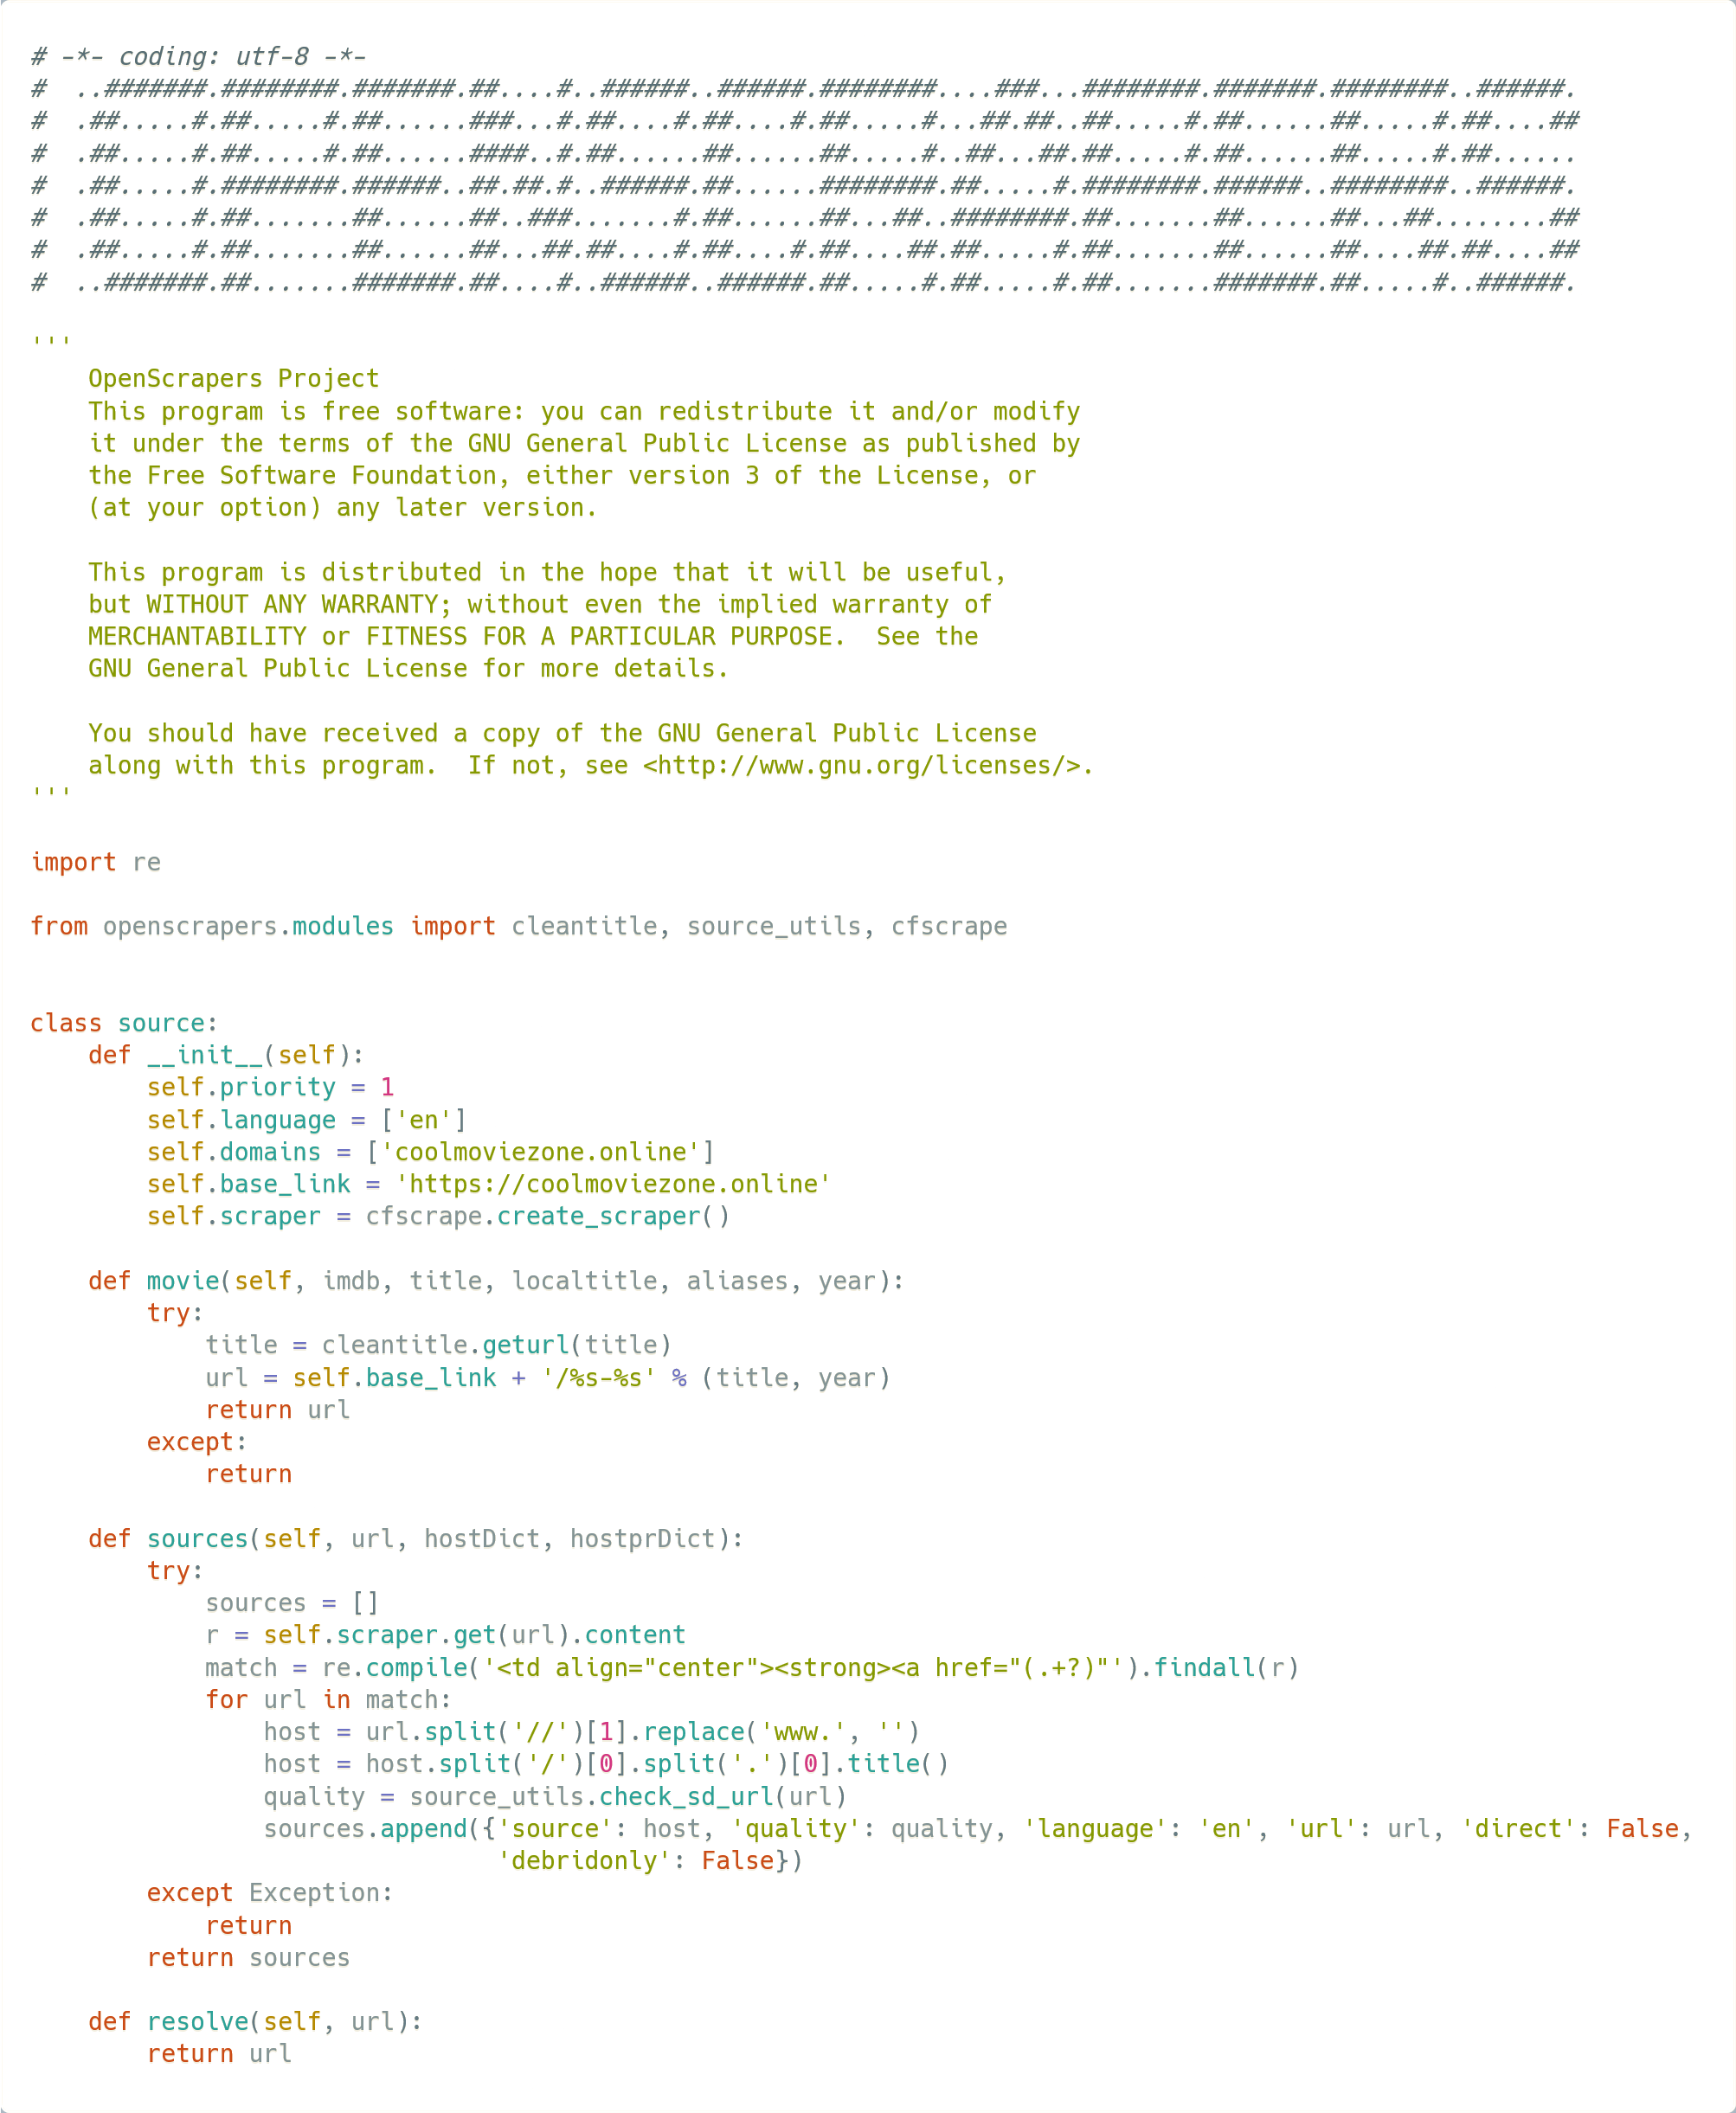
\includegraphics[width=0.8\textwidth]{img/CodeMirage/code example2.png}
    \caption{codemirage code example with large comment sections}
    \label{fig:codemirage example}
\end{figure}

The proposed methods to detect LLM generated code
vary significantly in their approaches: for example, 
"Codevision: Detecting llm-generated code using 2d token probability 
maps and vision models."\cite{xu2025codevision} treats 
source code as an image and employs convolutional neural networks (CNNs), 
"Uncovering llm-generated code: A zero-shot synthetic code detector via code rewriting."
\cite{ye2025uncovering} and 
"Distinguishing llm-generated from human-written code by contrastive learning" 
\cite{xu2025distinguishing} use models trained by contrastive learning, 
while "Spotting llms with binoculars: Zero-shot detection of machine-generated text" 
\cite{hans2024spotting}
and "Between lines of code: Unraveling the distinct patterns of machine and human programmers" 
\cite{shi2024between} propose zero-shot techniques inspired 
by the well known machine generated text detector DetectGPT\cite{mitchell2023detectgpt} 
and "Detection of LLM-Generated Java Code Using Discretized Nested Bigrams" \cite{paek2024detection}
introduces novel 
discretized syntactic features to classifying.

There is also variation in the scope of these works. 
Certain methods are limited to detecting code from a single LLM—such as 
"Automatic detection of llm-generated code: A case study of claude 
3 haiku."\cite{anthropic2024model} focusing on Claude 3, 
or "Chatgpt code detection: Techniques for uncovering the source of code." 
\cite{oedingen2024chatgpt} on GPT. 
Additionally, some studies restrict their analysis to a single programming 
language (typically Python), whereas others extend it to multiple 
languages, commonly including C++ and Java.

Despite the variety of methods and works proposed, 
most of these papers are still in a pre-publication state. 
Some report overly optimistic results, others have \textbf{not released the 
code or models presented in their work}, and others have released only 
part of the work.
For this reason, despite the existence of several methods 
proposed in the literature with more than positive performance, 
\textbf{it will only be possible to evaluate a limited set}.

It is also important to note that many papers in the literature address 
related but distinct problems, such as watermarking 
(e.g., "Codeip: A grammar-guided multi-bit watermark for large language 
models of code"\cite{guan2024codeip}, 
"Marking Code Without Breaking It: Code Watermarking for 
Detecting LLM-Generated Code" \cite{kim2025marking}, 
"Robust and secure code watermarking for large 
language models via ml/crypto codesign" \cite{zhang2025robust}, 
and "Detection of llm-paraphrased code and identification of the 
responsible llm using coding style features" \cite{park2025detection}) 
or plagiarism detection where the modification 
is performed by an LLM (e.g., "Detection of llm-paraphrased code and 
identification of the responsible llm using coding style features" 
\cite{park2025detection}). These lines of 
research, while relevant, do not directly solve the detection problem 
addressed in this thesis. This variety of objectives and approaches 
clearly reflects the dynamic and evolving nature of the field, reinforcing 
the need for a solid, comparative foundation on which to build a functional 
and user-oriented detection system.


